\problemname{Monopol}

Jocke och hans vänner brukar spela Monopol med varandra. Men efter otaliga spel har de tröttnat
på de vanliga reglerna, och har därför ändrat på dem en aning:


Först väljer de ett lagom stort land. De tar sedan en titt på vägnätet i landet och väljer ut ett
antal städer som bildar en cykel (som på ett monopolbräde). Därefter åker de till landet, och spelar
genom att åka runt cykeln i sina bilar och köper/säljer fastigheter med riktiga pengar.


Det finns dock en begränsning som gör det svårt att genomföra spelet: de måste hitta en lämplig
cykel i vägnätet. Vissa länder har nämligen väldigt stora vägnät. Något som försvårar ytterligare är 
att cykeln måste ha ett jämnt antal kanter, för annars funkar inte reglerna (``Fri parkering'' hamnar inte
i mitten vilket ger ett obalanserat spel).


Du får givet en oriktad graf, och din uppgift är att hitta en cykel med ett jämnt antal kanter, 
om det finns en.

\begin{figure}[!h]
\begin{center}
  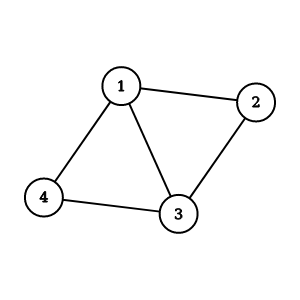
\includegraphics[width=5cm]{sample1.png}
  \quad
  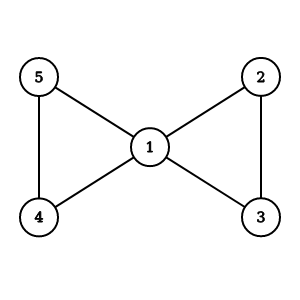
\includegraphics[width=5cm]{sample2.png}
  \quad
  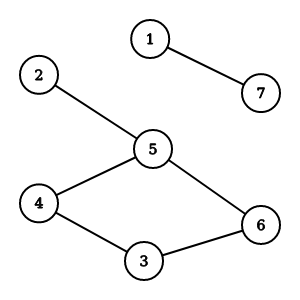
\includegraphics[width=5cm]{sample3.png}
\end{center}
  \caption{Illustration av graferna i de tre exempelfallen.}
\end{figure}

\section*{Indata}

Den först raden innehåller två heltal $N$ och $M$, antalet noder respektive antalet kanter
($1\le N \le 10^5$, $0\le M \le \mathrm{min}(2\cdot 10^5, \tfrac{n(n-1)}{2})$).

Sedan följer $M$ rader med två heltal $a$ och $b$ vardera, vilket betyder att det finns en kant mellan noderna $a$ och $b$ i grafen ($1\le a, b \le N$ och $a\neq b$). Det är garanterat att det inte finns flera kanter mellan samma par av noder i grafen.

\section*{Utdata}
Om det inte finns en jämn cykel, skriv ut en rad med strängen ``\texttt{NO}''.

Om det finns en jämn cykel, skriv ut en rad med strängen ``\texttt{YES}''. Därefter ska du skriva ut en sådan cykel. Skriv först ut en rad med ett \textbf{jämnt} heltal $k$ ($4\le k \le N$), antalet noder i din cykel. På nästa rad, skriv ut $K$ stycken \textbf{olika} heltal $v_{1}, v_{2}, \ldots, v_{k}$ ($1\le v_{i}\le N$) separerade av mellanslag: noderna på din cykel, så att det kanterna $(v_{1},v_{2}), (v_{2},v_{3}),\ \ldots, (v_{k-1},v_{k}), (v_{k}, v_{1})$ finns i grafen.

Om det finns flera möjliga svar så kommer vilket som helst accepteras.

\section*{Poängsättning}
Din lösning kommer att testas på en mängd testfallsgrupper.
För att få poäng för en grupp så måste du klara alla testfall i gruppen.

\noindent
\begin{tabular}{| l | l | l |}
  \hline
  Grupp & Poängvärde & Gränser \\ \hline \hline
  $1$ & 18 & $N\le 10$
  \\ \hline
  $2$ & 16 & $N\le 100$ och $M\le 200$
  \\ \hline
  $3$  & 17 & Grafen är bipartit
  \\ \hline
  $4$  & 13 & Alla noder i grafen har grad högst 2
  \\ \hline
  $5$  & 18 & Alla noder i grafen har grad minst 3
  \\ \hline
  $6$  & 18 & Inga ytterligare begränsningar
  \\ \hline
\end{tabular}

\noindent Notera att vissa exempelfall inte är giltiga i vissa testfallsgrupper.

\section*{Exempelfall}
